\chapter{Overview of FACEMC}
\label{ch:code_overview}
A professional software development process can be broken into five main phases:
the problem definition, the requirements analysis, the high-level design, 
construction, and system testing \citep{mcconnell_code_2004}. The first
three phases constitute the planning phase. They are considered the most 
important part of the development process \citep{mcconnell_code_2004}. 

The problem definition will not contain any reference to solution methods
but should clearly define the problem that the software will solve. The
problem definition for FACEMC was essentially given in the introduction and 
will therefore be neglected in this chapter. 

During the requirements analysis one determines what the scope of the system is 
and more generally, what the system is supposed to do 
\citep{mcconnell_code_2004}. Completion of the requirements analysis is the 
first step towards a solution to the problem definition. 

The high-level design or architecture identifies the subsystems and major 
classes and their interconnections that will allow for the requirements 
to be met. The architecture is very important because it determines the 
conceptual integrity of the software and provides guidance to programmers
\citep{mcconnell_code_2004}. 

The construction phase is the only phase where the software is actually written.
This phase will not be discussed further in this chapter. Though the system 
testing phase was listed last it does not only occur after the construction 
phase. A large part of this phase occurs in conjunction with the construction 
phase \citep{mcconnell_code_2004}. This phase is also very important and will 
be discussed in detail in one of the following sections. 

\section{Requirements}
While more detail is certainly better when outlining the code requirements since
they will lay the foundation for the entire code, only a brief discussion of
the requirement for FACEMC will be given. The requirements that will be 
discussed fall into the following categories:
\begin{itemize}
  \item user interface
  \item spatial domain modeling capabilities
  \item radiation modeling capabilities
  \item random number generation
  \item estimators
  \item variance reduction capabilities
  \item input file formats
  \item output file formats
  \item auxiliary capabilities
  \item parallelism
\end{itemize}

\subsection{User Interface}
The main user interface will be strictly a command-line interface (CLI). On the 
command-line, users will specify the necessary inputs, which will generally
refer the code to the required input files and the desired output files. 

\subsection{Spatial Domain Modeling Capabilities}
Two types of spatial domain modeling will be possible. The first type is based
on a combinatorial method where Boolean combinations of geometric surfaces of 
order two or less are specified in order to create volumes. This modeling 
capability will be very similar to the one in MCNP5
\citep{x-5_monte_carlo_team_mcnp_2003}. Implementation details of this method 
can be found in the report by Hendricks \citep{hendricks_calculation_1980}. 
The second type of spatial domain modeling is computer-aided drafting (CAD) 
based and will rely on the direct accelerated geometry (DAG) package in the 
mesh-oriented database (MOAB) 
\citep{tautges_acceleration_2009, tautges_moab:_2004}. This modeling capability 
will allow for any types of surface to be modeled. Its use will also be 
contingent on the users accesses to another code called CUBIT, which is not 
open source \citep{blacker_cubit_1994}. 

\subsection{Radiation Modeling Capabilities}
As mentioned in the introduction, the types of radiation that the code will be 
able to model will be photons in the energy range of one keV to twenty MeV and 
neutrons in the energy range of $10^{-5}$ eV to twenty MeV. Adjoint photons and 
adjoint neutrons in the same energy ranges will also be able to be modeled. 
The code will not be able to model charged particles. The physics that 
describes the interaction of the radiation with a material will be as detailed
as possible. However, the user will have the option to select less detailed
physics if speed is more important than accuracy. 

To model photons and neutrons two cross section libraries will be used. For
photons, the 1997 evaluated photon data library (EPDL97) will be used 
\citep{cullen_epdl97_1997}. For neutrons, the seventh version of the evaluated 
nuclear data library (ENDF/B-VII.1) will be used 
\citep{chadwick_endf/b-vii.1_2011}. While both of these libraries are text 
files, the Cross Section Evaluation Working Group has expressed interest 
in storing future versions of the ENDF/B data library in the binary HDF5 format 
\citep{mattoon_generalized_2012}. Therefore, all processed cross section data
will be stored in HDF5 format in order to be prepared for future versions of
the cross section libraries. 

\subsection{Random Number Generation}
Uniform random number generation is an integral part of the Monte Carlo random
walk process. The linear congruential generator must be available due to its
success in MCNP and many other Monte Carlo codes \citep{brown_mcnp5_2002}. 
Other random number generators will also be available in order to test their
speed in relation to the linear congruential generator.

\subsection{Estimators}
The collision estimator and the track length estimator will be available for 
the user to gather information about his or her model. No expected value 
estimators, such as the point detector, will be available. Many options will be 
available to further refine the behavior of these estimators. These options 
include phase space binning and for collision estimators, collision number 
binning. The known function which defines the estimator can be either a user 
defined function specified in the input file or a cross section present in the 
cross section library. The user will also have the ability to define new 
functions based on combinations of the previous two through basic mathematical 
operations. 

\subsection{Variance Reduction}
In order to be able to generate results in a reasonable amount of time for
deep penetration problems, which are commonly encountered, variance reduction 
techniques will have to be available. Only five commonly used techniques will
be available in FACEMC. These techniques are implicit capture, Russian roulette,
splitting, forced collision, and weight windows. If the weight window technique
is used, the user will be in charge of supplying an appropriate weight window
mesh. A weight window generator will not be available in FACEMC.

\subsection{Input File Formats}
All input files other than the files that describe the CAD geometries will be
in extensible markup language (XML) format. This decision was made because of
the availability of XML parsers and because of the complexity involved in
creating generic text file readers (based on previous experience). Further,
two input files will always be necessary. One will describe the spatial domain 
and the other will describe all other details of the problem.

\subsection{Output File Formats}
All output files will also be written to XML files except when certain 
estimators with large phase space binning are used, in which case a 
Visualization ToolKit (VTK) file will be written. The VTK file format was 
chosen because of its compatibility with many visualization codes.

\subsection{Parallelism}
The code must also be able to run in parallel in order to solve larger and 
more complex problems. While several parallel algorithms exist that can be
used in Monte Carlo codes, the hierarchical parallelism algorithm found in
the paper by Brunner and Brantley will be implemented 
\citep{brunner_efficient_2009}. Their algorithm allows for domain decomposition,
however, only domain replication\footnote{Domain replication is where each 
processor receives a copy of the problem model. The maximum problem size is
therefore limited by the processor with the smallest amount of memory
available.} will be allowed. The message passing interface (MPI) will be used
to implement the algorithm.

\section{High-Level Design}
To meet the requirements that were outlined in the previous section, several
subsystems and major classes have been identified. The three main subsystems 
are the initialization subsystem, the problem simulation subsystem and the 
spatial domain plotting subsystem. These subsystems and their major components 
are shown in figures \ref{fig:initialization}, \ref{fig:problem_simulator} and 
\ref{fig:spatial_domain_plotter}. A simple line between two components 
indicates that a component contains another component. The color of the two 
components will also be different to indicate the component hierarchy. A black 
arrow between two components in the same level of the hierarchy indicates the 
information flow between the two components. A red arrow between two components 
indicates that one component creates another component.
\begin{figure}[t!]
  \begin{center}
    \scalebox{0.7}{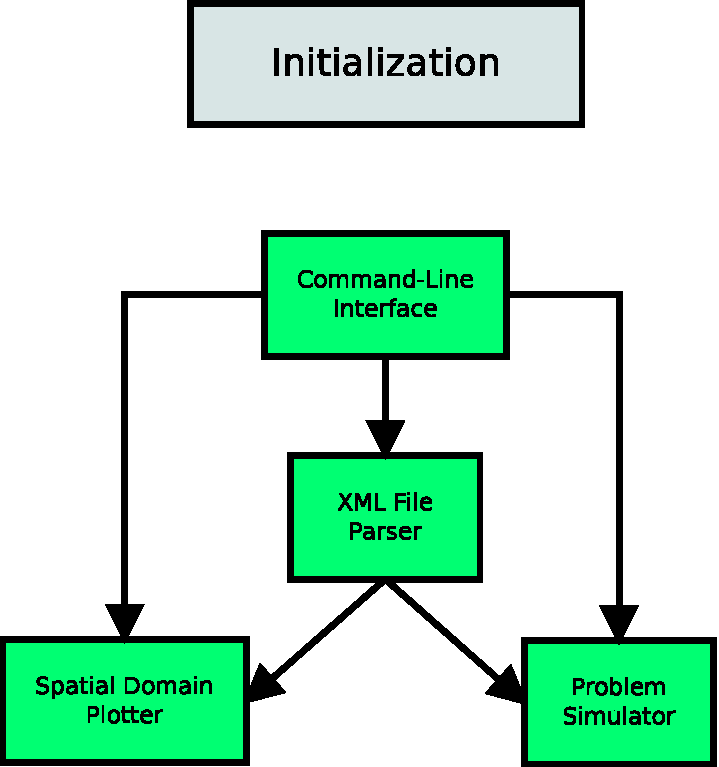
\includegraphics{chapters/code_overview/Initialization.pdf}}
  \end{center}
  \caption{\textbf{Initialization Subsystem.}
    \textit{The initialization subsystem consists of two major classes and
      two other subsystems. The two classes are the command-line interface
      and the XML file parser. The two subsystems are the spatial domain
      plotter and the problem simulator. Depending on the requests made by
      the user, either the problem simulator or the spatial domain plotter
      will be initialized.}}
  \label{fig:initialization}
\end{figure}
\begin{figure}[t!]
  \begin{center}
    \scalebox{0.7}{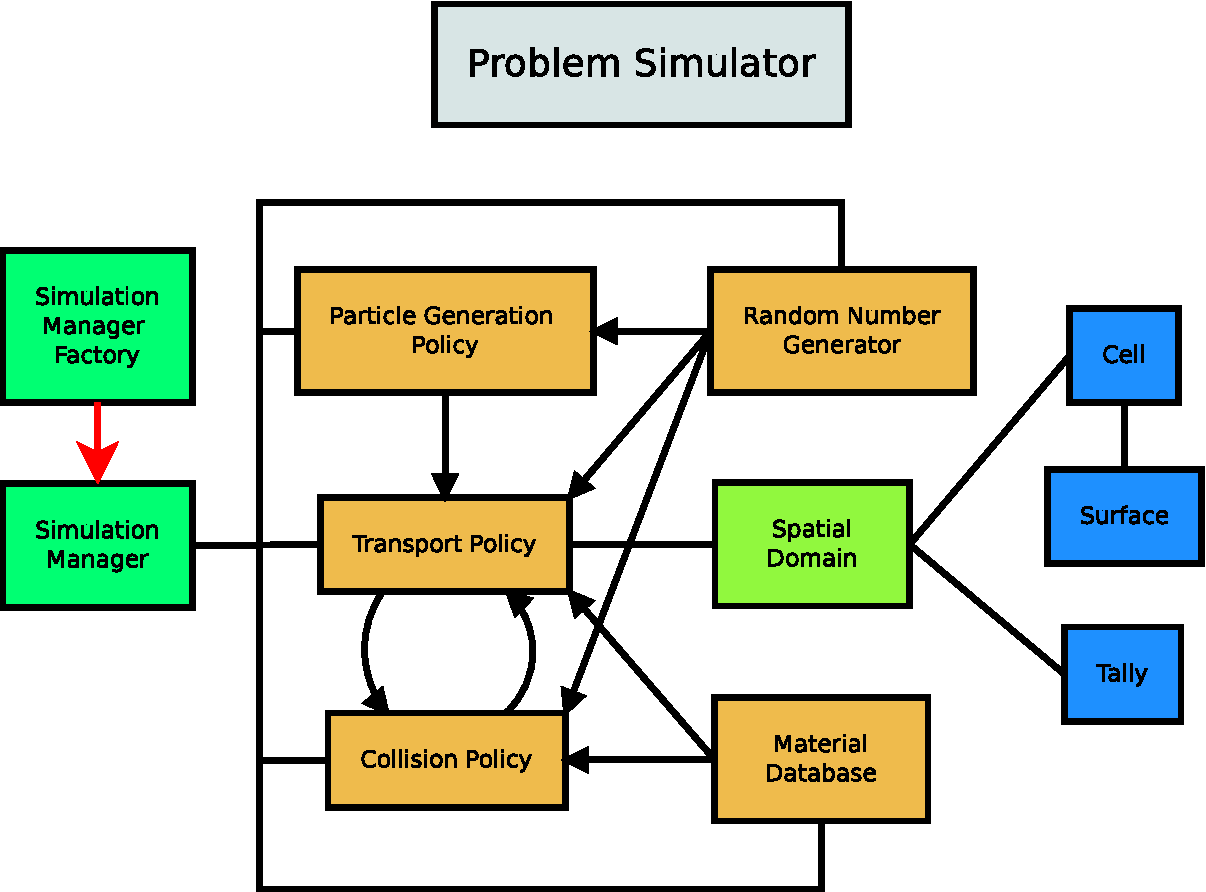
\includegraphics{chapters/code_overview/Problem_Simulator.pdf}}
  \end{center}
  \caption{\textbf{Problem Simulation Subsystem.}
    \textit{The problem simulation subsystem consists of several major classes.
      Based on the user inputs pulled from the XML file(s), the simulation
      manager factory will create the necessary simulation manager. The 
      simulation manager will control the simulation of particles based on
      three policy classes: the particle generation policy, the transport
      policy, and the collision policy. The transport policy will contain
      the spatial domain class, which will contain all cells, surfaces and
      tallies.}}
  \label{fig:problem_simulator}
\end{figure}
\begin{figure}[t!]
  \begin{center}
    \scalebox{0.7}{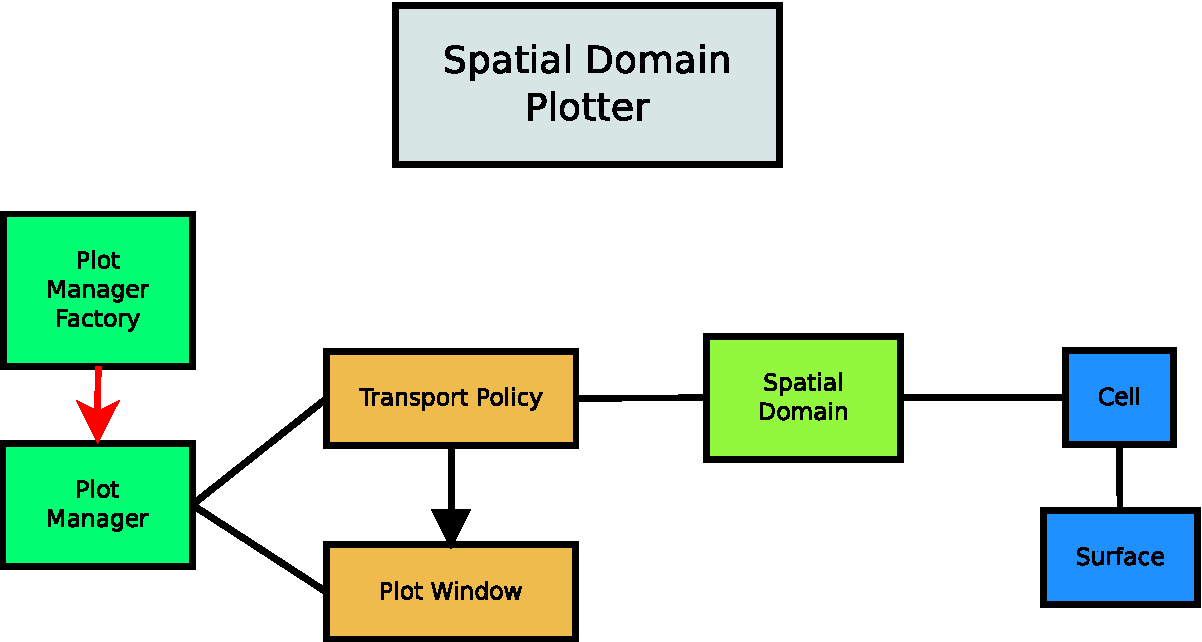
\includegraphics{chapters/code_overview/Spatial_Domain_Plotter.pdf}}
  \end{center}
  \caption{\textbf{Spatial Domain Plotting Subsystem.}
    \textit{The spatial domain plotting subsystem consists of several major
      classes. Based on the user inputs pulled from the XML file(s), the 
      plot manager factory will create the necessary plot manager. The plot
      manager will control how the spatial domain is plotted based on two
      classes: the transport policy, which is also a part of the simulation 
      manager, and the plot window. The transport policy will primarily be used
      to visualize the spatial domain through ray-tracing.}}
  \label{fig:spatial_domain_plotter}
\end{figure}

The first version of these components except for the XML parser and the geometry
plotter are currently completed. The second version of several of these 
components are also currently completed. The second versions of these 
components will incorporate lessons learned from the first versions in addition 
to better programming practices. 

\section{System Testing: Verification and Validation}
System testing can be broken into two components: verification and validation. 
Verification, which is the process of determining whether or not particular 
components of the software fulfill a set of established requirements, occurs
in conjunction with the construction phase \citep{procassini_verification_2004}.
Verification is accomplished with an on-going process of unit 
testing\footnote{A unit test is written for one component of the code and test 
that expected outputs are returned for a set of inputs.} during the 
construction phase. Verification of FACEMC through unit testing will not be 
discussed in this chapter. 

Validation, which is the process of determining whether the software returns
correct results for desired quantities, occurs at the end of the software 
development process. For FACEMC, the following validation plan has been created 
to ensure that the code functions properly:
\begin{enumerate}
  \item Calculation of benchmark test problems for photons and neutrons
  \item Code-to-code comparisons of integral quantities and photon or neutron 
    spectra against other Monte Carlo codes that have been previously validated
  \item Comparison of integral quantities and spectra from forward and reverse
    simulations
\end{enumerate}

\subsection{Validation Step 1}
The first step of the validation plan will compare results from FACEMC forward
simulations against data from benchmark test problems. For photons, the same
problem that was used to validate GEANT4 photon simulations will be used 
\citep{amako_comparison_2005}. Figure \ref{fig:photon_benchmark_problem} shows 
the problem set up.
\begin{figure}[t!]
  \begin{center}
    \scalebox{0.7}{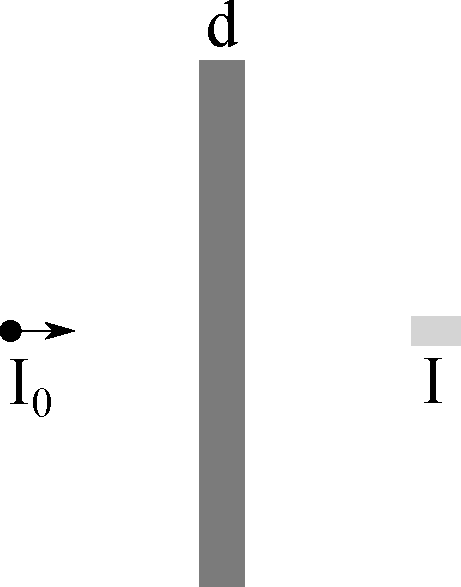
\includegraphics{chapters/code_overview/photon_benchmark_problem.pdf}}
  \end{center}
  \caption{\textbf{Photon Benchmark Problem.}
    \textit{A monoenergetic beam of photons is directed at a slab of thickness
      d. The current of uncollided photons that exits the slab is calculated.}}
  \label{fig:photon_benchmark_problem}
\end{figure}
In this problem, photon mass attenuation coefficients and partial interaction
coefficients will be calculated at an array of energies and for a variety of 
materials. The values that are calculated will then be compared to the values 
from the National Institute of Standards and Technology  (NIST) XCOM database 
\citep{amako_comparison_2005}. The mass attenuation coefficient can be 
calculated with the following formula:
\begin{equation}
  \left(\frac{\mu}{\rho}\right) = -\frac{1}{\rho d}
  \ln{\left(\frac{I}{I_0}\right)}.
\end{equation}
If only a single reaction type is considered, the above equation can be used
to determine the partial interaction coefficient corresponding to the reaction
considered.

For neutrons, several experiments from the Shielding Integral Benchmark 
Archive Database (SINBAD) will be modeled and the resulting data will be 
compared to the experimental data in the database \citep{kodeli_sinbad_2006}.
The exact problems that will be modeled have not been determined yet.

\subsection{Validation Step 2}
The second step of the validation plan will focus on code-to-code comparisons
against other Monte Carlo codes that have been previously validated. Only a
single problem, which is shown in figure \ref{fig:code_comparison_problem} will 
be used in this step of the validation plan. 
\begin{figure}[t!]
  \begin{center}
    \scalebox{0.5}{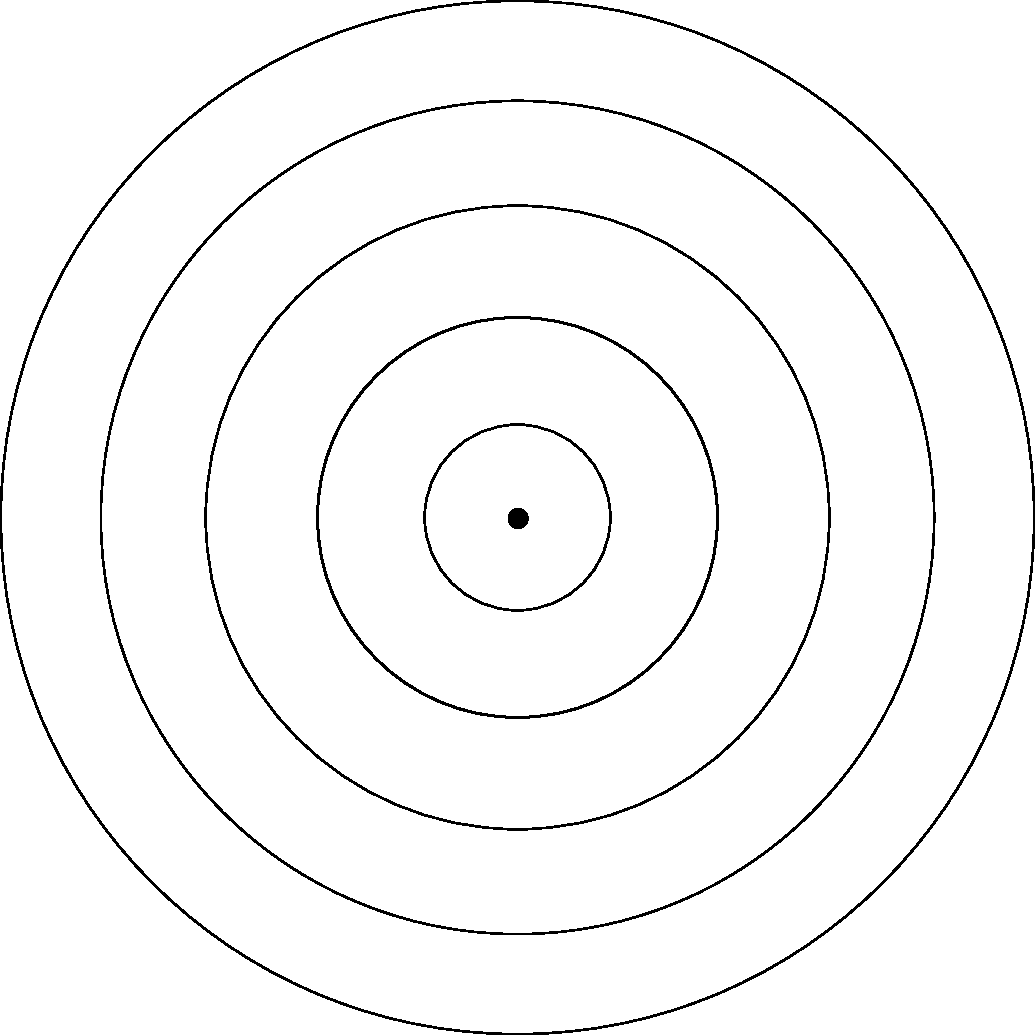
\includegraphics{chapters/code_overview/code_comparison_problem.pdf}}
  \end{center}
  \caption{\textbf{Code-to-Code Comparison Problem.}
    \textit{An isotropic point source is located at the center of five 
      concentric spheres. The radii of the spheres are 10 cm, 20 cm, 30 cm, 40
      cm and 50 cm. The spatial domain extends to infinity in every dimension.
      Only a single material is present throughout the spatial domain and there
      are no voids. Surface flux estimators are used on each sphere.}}
  \label{fig:code_comparison_problem}
\end{figure}
The spatial domain is an infinite medium containing a point source at the 
center of five concentric spheres. Two surface flux estimators are used at each
spherical surface. The first is used to estimate the total flux
at the surface and the second is discretized in energy so that the energy
spectrum of the particles crossing the surface can be estimated.

For photons, an isotropic point source with two discrete energies will
be modeled. For neutrons, an isotropic point source with a fission spectrum 
will be modeled. An array of materials will also be used to ensure that cross 
sections have been processed correctly. 

Two codes will be used to conduct the comparison for photons: MCNP5 and 
PENELOPE. Two codes will also be used to conduct the comparison for neutrons:
MCNP5 and TART2005. 

\subsection{Validation Step 3}
The third step of the validation plan will focus on comparisons between forward
and reverse calculations done using FACEMC only. After the second step of the
validation plan is complete the forward simulation mode can be deemed 
validated. It can therefore be used to validate the adjoint simulation mode. 

The same problem that was used in the second step of the validation
plan, shown in figure \ref{fig:code_comparison_problem}, will be used in this
step. Interestingly, the unique symmetry of this problem allows the reverse
problem to be constructed identically to the forward problem. A proof of this
symmetry is rather complex and requires the use of Green's functions 
\citep{bell_nuclear_1979}. It will therefore not be shown.

One case for photons has already been completed\footnote{This case was completed
before the validation plan was developed, which is why it was done out of 
order.}. The material that is present is water and the two discrete source
energies are 661.66 keV and 321.0 keV. The first discrete source energy
corresponds to the primary Cs-137 decay line and the second discrete source 
energy is contrived. Figures \ref{fig:val_plan_s3_c0_spectrum_diffs_water} and
\ref{fig:val_plan_s3_c0_spectrum_water} show the spectrum results for this
case.  From the figures, it is clear that the spectra calculated using the
forward and adjoint capabilities of FACEMC are in good agreement. 
\begin{figure}[t!]
  \begin{center}
    \scalebox{1.0}{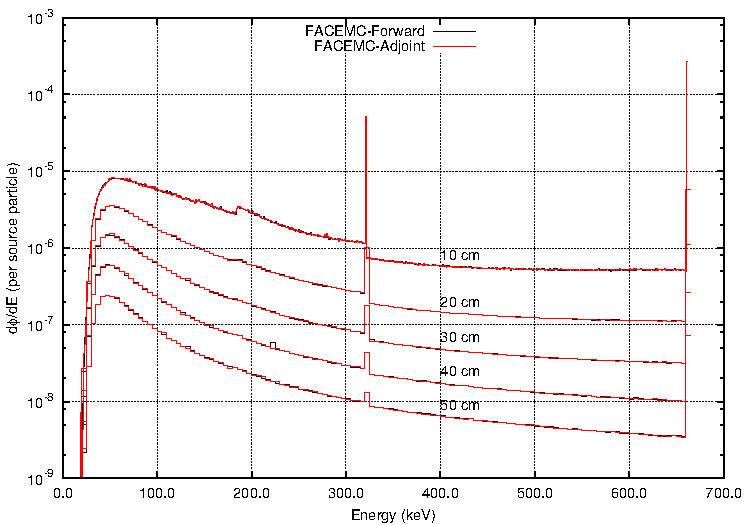
\includegraphics{chapters/code_overview/photon_spectrum_validation_comparison.pdf}}
  \end{center}
  \caption{\textbf{Validation Plan Step 3 - Case 0: Photon Spectra in Water.}
    \textit{The photon spectra computed using the forward and adjoint
      mode of FACEMC appear to be in very good agreement at all 
      surfaces of interest. All relative errors are less than 1.5\%.}}
  \label{fig:val_plan_s3_c0_spectrum_water}
\end{figure}
\begin{figure}[t!]
  \begin{center}
    \scalebox{1.0}{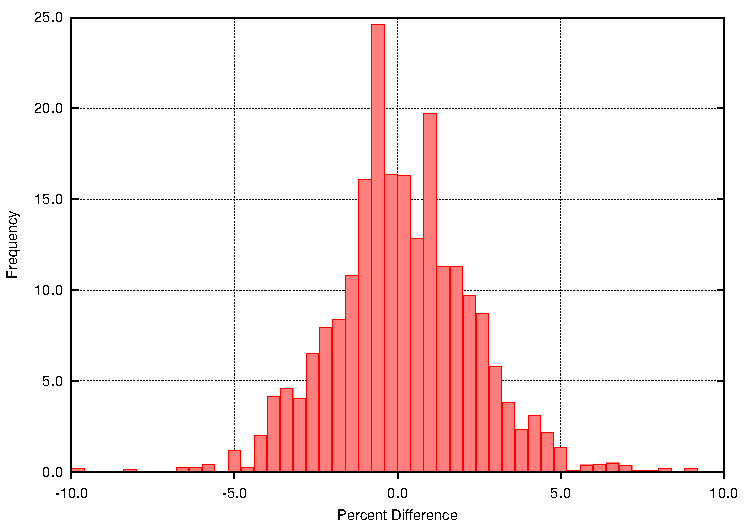
\includegraphics{chapters/code_overview/photon_spectrum_validation_comparison_difference.pdf}}
  \end{center}
  \caption{\textbf{Validation Plan Step 3 - Case 0: Photon Spectra Differences
      at 10 cm.}
    \textit{This plot shows the percent difference between each bin of the
      spectrum at 10 cm computed using the forward mode of FACEMC and each bin
      of the spectrum at 10 cm computed using the adjoint mode of FACEMC. The 
      majority of the percent differences are between -5.0\% and 5.0\%.}}
  \label{fig:val_plan_s3_c0_spectrum_diffs_water}
\end{figure}
Table \ref{table:val_plan_s3_c0_flux_water} shows the total flux results
for this case. The total flux calculated with the forward and adjoint modes are
also in very good agreement.
\begin{table}[ht]
  \caption{\textbf{Validation Plan Step 3 - Case 0: Photon Total Flux in Water.}
    \textit{The photon total flux computed using the forward and adjoint
      mode of FACEMC are in very good agreement at all surfaces of
      interest.}}
  \centering
  \begin{tabular}{c c c c c c}
    \hline\hline
    Distance & Flux & Relative & Flux & Relative & \% Diff. \\ 
    (cm) & (forward mode) & Error & (adjoint mode) & Error &  \\ [0.5ex]
    \hline
    10 & 1.5748e-3 & 0.0007 & 1.5788e-3 & 0.0014 & 0.25 \\
    20 & 4.1291e-4 & 0.0007 & 4.1491e-4 & 0.0018 & 0.48 \\
    30 & 1.4150e-4 & 0.0007 & 1.4235e-4 & 0.0022 & 0.60 \\
    40 & 5.2255e-5 & 0.0011 & 5.2322e-5 & 0.0027 & 0.13 \\
    50 & 1.9963e-5 & 0.0014 & 2.0030e-5 & 0.0033 & 0.34 \\ [1ex]
    \hline
  \end{tabular}
  \label{table:val_plan_s3_c0_flux_water}
\end{table}

An interesting take away from table \ref{table:val_plan_s3_c0_flux_water},
which is unrelated to the validation of the code, is that the current 
implementation of the adjoint mode is more costly to run than the implementation
of the forward mode. Even when the same number of particles are modeled the 
relative error of the adjoint mode is higher than the forward mode. This is 
solely a result of the properties of the adjoint weight factor, which were 
described in the previous chapter, given that the problem is modeled 
identically in both the forward and adjoint modes. Hoogenboom has described
some methods that could potentially ameliorate this issue 
\citep{hoogenboom_adjoint_1977}.
